\appendix

\section{Anhang: Erg�nzende Projektvereinbarungen}

\subsection{Projektorganisation}

\begin{tabular}{|l|l|}
\hline
Projektteam      &  M. Bigler (biglm2@hta-bi.bfh.ch) \\
                 &  S. R�ss (rasss@hta-bi.bfh.ch) \\
                 &  L. Zbinden (zbinl@hta-bi.bfh.ch) \\
\hline
Projektleiter    &  S. R�ss (rasss@hta-bi.bfh.ch) \\
\hline
Projektbetreuer  &  J.-P. Dubois (doj@hta-bi.bfh.ch) \\
                 &  C. Fuhrer (frc@hta-bi.bfh.ch) \\
\hline
\end{tabular}

\begin{figure}[h]
  \begin{center}
    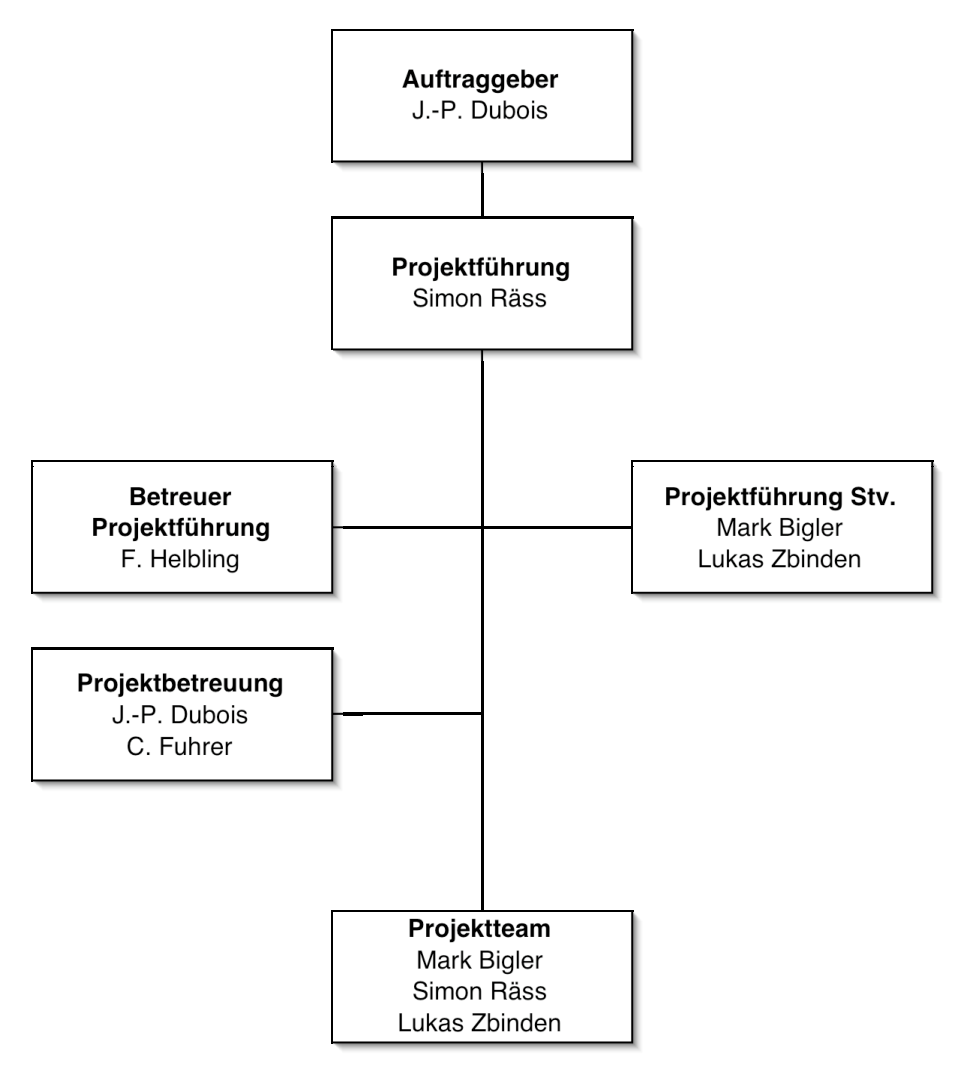
\includegraphics[width=10cm,height=9.2cm]{../../images/organigramm.eps}
  \end{center}
  \caption{Projektorganisation}
  \label{Projektorganisation}
\end{figure}


\subsection{Projektplanung}

\begin{table}
 \begin{tabular}{|l|l|}
  \hline
  Anfang der Semesterarbeit       &    21.02.2005 \\
  \hline
  Beginn der Initialiserungsphase &    21.02.2005 \\
  \hline
  Ende der Semesterarbiet         &    24.07.2005 \\
  \hline
 \end{tabular}
 \caption{Projektplanung}
 \label{Projektplanung}
\end{table}

\subsection{Qualit�tssicherung}

\subsection{Konfigurationsmanagement}
Es werden s�mtliche Dokumente des Projektmanagements, s�mtlicher Quellcode, die Inhalte der Website und die f�r die Erstellung des Programms ben�tigten externen Bibliotheken werden unter das Konfigurationsmanagement gestellt.

Die Projektdokumentation und Produktdokumentationen werden mit einer Versionskontrolle versehen. Die Dokumente k�nnen dabei die in der Tabelle \ref{Versionsnummern} angegebenen Zust�nde annehmen.

\begin{table}[!h]
\begin{tabular}{|l|l|}
\hline
Version     &  Bezeichnung \\
\hline
0.1 - 0.99  &  Entwurfsversionen \\
\hline
1.0         &  erste Release Version \\
\hline
1.1         &  allf�llige �berarbeitete Versionen \\
\hline
\end{tabular}
\caption{Versionsnummern}
\label{Versionsnummern}
\end{table}

F�r das Konfigurationsmanagement wird unser eigens installiertes Subversion Repository verwendet. Das entsprechende Repository ist unter \texttt{http://ace.iserver.ch:81/repos/ace/} erreichbar. Aus der commit Nachricht soll erkenntlich sein, wenn die Versionsnummer des Dokumentes erh�ht wurde. 

\subsection{Sicherheit}
